\documentclass[openany]{book}
\usepackage{lmodern}
\usepackage{amssymb,amsmath}
\usepackage{ifxetex,ifluatex}
\usepackage{fixltx2e} % provides \textsubscript
\ifnum 0\ifxetex 1\fi\ifluatex 1\fi=0 % if pdftex
  \usepackage[T1]{fontenc}
  \usepackage[utf8]{inputenc}
\else % if luatex or xelatex
  \ifxetex
    \usepackage{mathspec}
  \else
    \usepackage{fontspec}
  \fi
  \defaultfontfeatures{Ligatures=TeX,Scale=MatchLowercase}
\fi
% use upquote if available, for straight quotes in verbatim environments
\IfFileExists{upquote.sty}{\usepackage{upquote}}{}
% use microtype if available
\IfFileExists{microtype.sty}{%
\usepackage{microtype}
\UseMicrotypeSet[protrusion]{basicmath} % disable protrusion for tt fonts
}{}
\usepackage[margin=1in]{geometry}
\usepackage{hyperref}
\hypersetup{unicode=true,
            pdftitle={DATA 624: Project 1 - Part B},
            pdfauthor={Sang Yoon (Andy) Hwang \& Vinicio Haro},
            pdfborder={0 0 0},
            breaklinks=true}
\urlstyle{same}  % don't use monospace font for urls
\usepackage{natbib}
\bibliographystyle{plainnat}
\usepackage{color}
\usepackage{fancyvrb}
\newcommand{\VerbBar}{|}
\newcommand{\VERB}{\Verb[commandchars=\\\{\}]}
\DefineVerbatimEnvironment{Highlighting}{Verbatim}{commandchars=\\\{\}}
% Add ',fontsize=\small' for more characters per line
\usepackage{framed}
\definecolor{shadecolor}{RGB}{248,248,248}
\newenvironment{Shaded}{\begin{snugshade}}{\end{snugshade}}
\newcommand{\KeywordTok}[1]{\textcolor[rgb]{0.13,0.29,0.53}{\textbf{#1}}}
\newcommand{\DataTypeTok}[1]{\textcolor[rgb]{0.13,0.29,0.53}{#1}}
\newcommand{\DecValTok}[1]{\textcolor[rgb]{0.00,0.00,0.81}{#1}}
\newcommand{\BaseNTok}[1]{\textcolor[rgb]{0.00,0.00,0.81}{#1}}
\newcommand{\FloatTok}[1]{\textcolor[rgb]{0.00,0.00,0.81}{#1}}
\newcommand{\ConstantTok}[1]{\textcolor[rgb]{0.00,0.00,0.00}{#1}}
\newcommand{\CharTok}[1]{\textcolor[rgb]{0.31,0.60,0.02}{#1}}
\newcommand{\SpecialCharTok}[1]{\textcolor[rgb]{0.00,0.00,0.00}{#1}}
\newcommand{\StringTok}[1]{\textcolor[rgb]{0.31,0.60,0.02}{#1}}
\newcommand{\VerbatimStringTok}[1]{\textcolor[rgb]{0.31,0.60,0.02}{#1}}
\newcommand{\SpecialStringTok}[1]{\textcolor[rgb]{0.31,0.60,0.02}{#1}}
\newcommand{\ImportTok}[1]{#1}
\newcommand{\CommentTok}[1]{\textcolor[rgb]{0.56,0.35,0.01}{\textit{#1}}}
\newcommand{\DocumentationTok}[1]{\textcolor[rgb]{0.56,0.35,0.01}{\textbf{\textit{#1}}}}
\newcommand{\AnnotationTok}[1]{\textcolor[rgb]{0.56,0.35,0.01}{\textbf{\textit{#1}}}}
\newcommand{\CommentVarTok}[1]{\textcolor[rgb]{0.56,0.35,0.01}{\textbf{\textit{#1}}}}
\newcommand{\OtherTok}[1]{\textcolor[rgb]{0.56,0.35,0.01}{#1}}
\newcommand{\FunctionTok}[1]{\textcolor[rgb]{0.00,0.00,0.00}{#1}}
\newcommand{\VariableTok}[1]{\textcolor[rgb]{0.00,0.00,0.00}{#1}}
\newcommand{\ControlFlowTok}[1]{\textcolor[rgb]{0.13,0.29,0.53}{\textbf{#1}}}
\newcommand{\OperatorTok}[1]{\textcolor[rgb]{0.81,0.36,0.00}{\textbf{#1}}}
\newcommand{\BuiltInTok}[1]{#1}
\newcommand{\ExtensionTok}[1]{#1}
\newcommand{\PreprocessorTok}[1]{\textcolor[rgb]{0.56,0.35,0.01}{\textit{#1}}}
\newcommand{\AttributeTok}[1]{\textcolor[rgb]{0.77,0.63,0.00}{#1}}
\newcommand{\RegionMarkerTok}[1]{#1}
\newcommand{\InformationTok}[1]{\textcolor[rgb]{0.56,0.35,0.01}{\textbf{\textit{#1}}}}
\newcommand{\WarningTok}[1]{\textcolor[rgb]{0.56,0.35,0.01}{\textbf{\textit{#1}}}}
\newcommand{\AlertTok}[1]{\textcolor[rgb]{0.94,0.16,0.16}{#1}}
\newcommand{\ErrorTok}[1]{\textcolor[rgb]{0.64,0.00,0.00}{\textbf{#1}}}
\newcommand{\NormalTok}[1]{#1}
\usepackage{graphicx,grffile}
\makeatletter
\def\maxwidth{\ifdim\Gin@nat@width>\linewidth\linewidth\else\Gin@nat@width\fi}
\def\maxheight{\ifdim\Gin@nat@height>\textheight\textheight\else\Gin@nat@height\fi}
\makeatother
% Scale images if necessary, so that they will not overflow the page
% margins by default, and it is still possible to overwrite the defaults
% using explicit options in \includegraphics[width, height, ...]{}
\setkeys{Gin}{width=\maxwidth,height=\maxheight,keepaspectratio}
\IfFileExists{parskip.sty}{%
\usepackage{parskip}
}{% else
\setlength{\parindent}{0pt}
\setlength{\parskip}{6pt plus 2pt minus 1pt}
}
\setlength{\emergencystretch}{3em}  % prevent overfull lines
\providecommand{\tightlist}{%
  \setlength{\itemsep}{0pt}\setlength{\parskip}{0pt}}
\setcounter{secnumdepth}{5}

%%% Use protect on footnotes to avoid problems with footnotes in titles
\let\rmarkdownfootnote\footnote%
\def\footnote{\protect\rmarkdownfootnote}

%%% Change title format to be more compact
\usepackage{titling}

% Create subtitle command for use in maketitle
\newcommand{\subtitle}[1]{
  \posttitle{
    \begin{center}\large#1\end{center}
    }
}

\setlength{\droptitle}{-2em}

  \title{DATA 624: Project 1 - Part B}
    \pretitle{\vspace{\droptitle}\centering\huge}
  \posttitle{\par}
    \author{Sang Yoon (Andy) Hwang \& Vinicio Haro}
    \preauthor{\centering\large\emph}
  \postauthor{\par}
      \predate{\centering\large\emph}
  \postdate{\par}
    \date{October 22, 2019}

\usepackage{booktabs}
\usepackage[table]{xcolor}

% set plain style for page numbers
\pagestyle{plain}
\raggedbottom

% change font
\usepackage{fontspec}
\setmainfont{Arial}

% remove "chapter" from chapter title
\usepackage{titlesec}
\titleformat{\chapter}
  {\normalfont\LARGE\bfseries}{\thechapter}{1em}{}
\titlespacing*{\chapter}{0pt}{3.5ex plus 1ex minus .2ex}{2.3ex plus .2ex}

% create color block quotes
\usepackage{tcolorbox}
\newtcolorbox{myquote}{colback=orange!05!white, colframe=black!75!black}
\renewenvironment{quote}{\begin{myquote}}{\end{myquote}}

% wrap text
\usepackage{geometry}[textwidth=6in]

% kable 
\usepackage{tabu}
\usepackage{float}
\usepackage{booktabs}
\usepackage{longtable}
\usepackage{array}
\usepackage{multirow}
\usepackage{wrapfig}
\usepackage{float}
\usepackage{colortbl}
\usepackage{pdflscape}
\usepackage{tabu}
\usepackage{threeparttable}
\usepackage{threeparttablex}
\usepackage[normalem]{ulem}
\usepackage{makecell}
\usepackage{xcolor}

\begin{document}
\maketitle

{
\setcounter{tocdepth}{1}
\tableofcontents
}
\chapter*{Part B: Forecasting Power}\label{part-b}
\addcontentsline{toc}{chapter}{Part B: Forecasting Power}

\begin{quote}
\textbf{Instructions:} Part B consists of a simple dataset of
residential power usage for January 1998 until December 2013. Your
assignment is to model these data and a monthly forecast for 2014. The
data is given in a single file. The variable `KWH' is power consumption
in Kilowatt hours, the rest is straight forward. Add these to your
existing files above - clearly labeled.
\end{quote}

\section*{Exploration}\label{b-exploration}
\addcontentsline{toc}{section}{Exploration}

From our time series data (frequency = 12, monthly power\_data) we
observed there is a missing value in September 2008. We used imputation
method called na.interpolation which performs a technique in numerical
analysis which estimates a value from known data points. For our case,
linear method using first order Taylor polynomial is used.

Our initial time series plot reveal annual seasonality within this time
series. The box plot/seasonality plot actually reveals where power
consumption fluctuations occur within each of the cycke positions. We
can speculate that this could be due to there being no major Holidays
that require power draining decor plus we assume minimal AC usage during
the cold months.

We see power consumption increase between the months of June and August.
This must be tied to AC usage during the warmer months of a year and
finally power usage dips from September to Novemeber with a small spike
in December. We speculate that thisis due to transitioning out of
summer. The spike in December could be connected to the usage or Holiday
lights being kept on.

Within the overall TS plot, we see a dip in July 2010. This could be due
to a power outtage during a hot summer month. This can certainly be
considered to be an outlier within this TS. Using TSOutliers, we can
actually identify the index where our outliers may be. TSoutliers also
replaces the outlier using Box-Cox. If set lambda=auto, then TSoutliers
will automatically perform Box-Cox transformation.

The ACF plot shows that autocorrelations are well outside the
significant space indicating the series is not white noise,
non-stationary.

\subsection{Series plot}\label{series-plot}

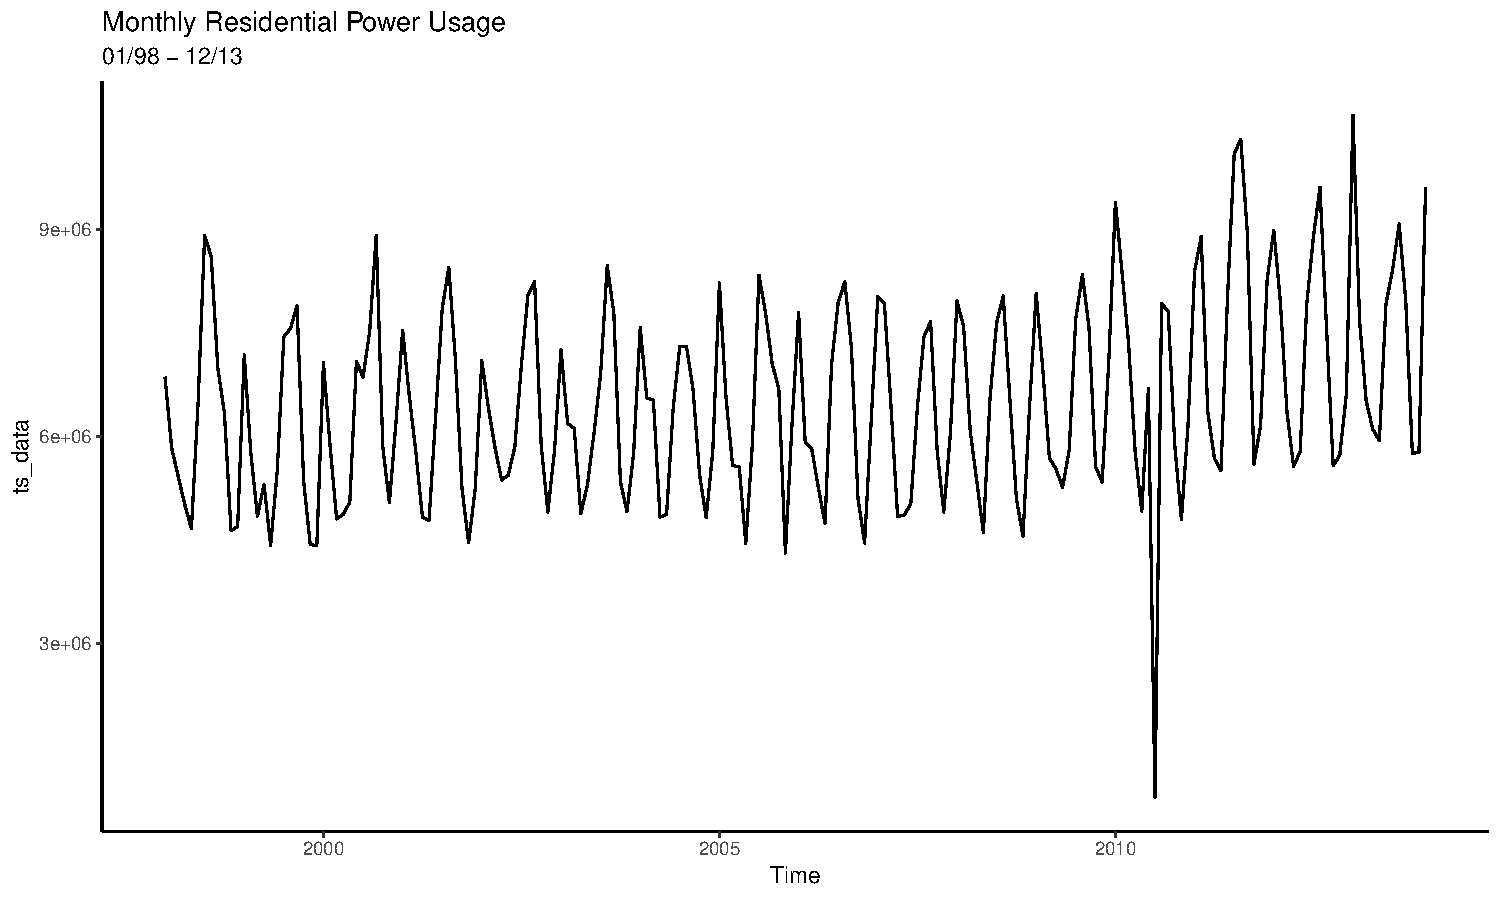
\includegraphics{Part-B-AS.final.firstparameter_files/figure-latex/unnamed-chunk-1-1.pdf}

\subsection{Seasonal plots}\label{seasonal-plots}

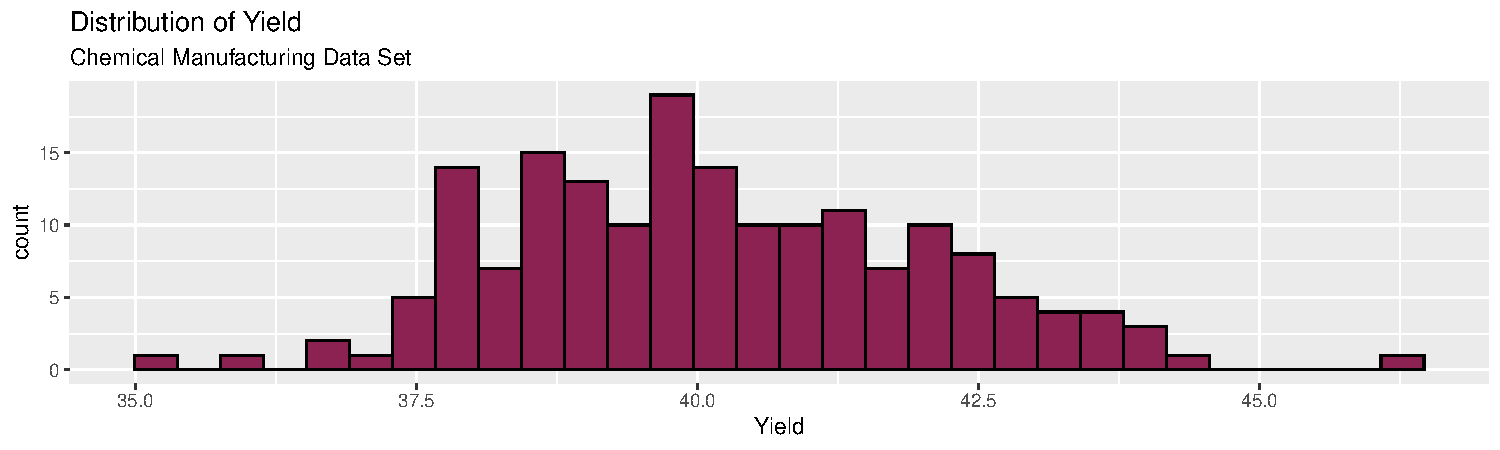
\includegraphics{Part-B-AS.final.firstparameter_files/figure-latex/unnamed-chunk-2-1.pdf}

\subsection{Diagnostic plots}\label{diagnostic-plots}

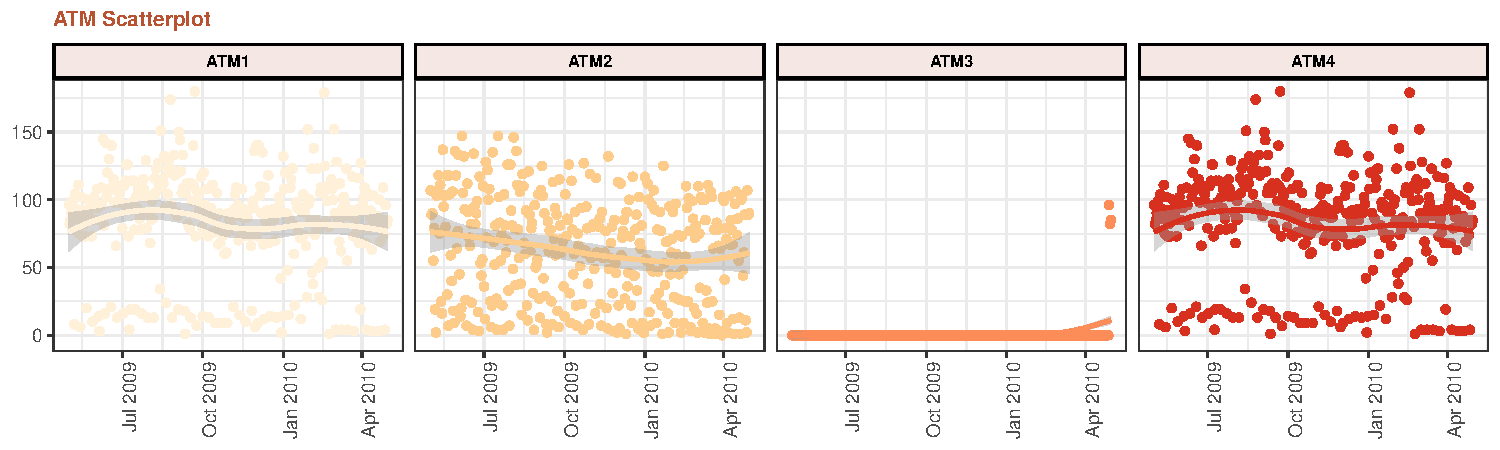
\includegraphics{Part-B-AS.final.firstparameter_files/figure-latex/unnamed-chunk-3-1.pdf}

\section*{Data Model}\label{b-model}
\addcontentsline{toc}{section}{Data Model}

Out of the models we built, we can make some preliminary observations.
The residuals for each of our models does not have a major deviance from
normality, however residuals of Model \#1: ARIMA do not have an extended
number of bins distorting the normality proximity but we can say it is
still fairly normally distributed.

The residual ACF plots show residual autocorrelations for each of our
models. Model \#1: ARIMA has less autocorrelation than the other three
models. Model 1 is well within the 95\% limits indicated by the dotted
blue lines.

If we examine the Ljung-Box test results for our models, the only model
with a p-value \textgreater{} 0.05 is Model \#1: ARIMA. This implies
that the residuals from other models are not independent, hence not
white noise. The full model summary can be viewed in the appendix.

\subsection{Model \#1: ARIMA}\label{model-1-arima}

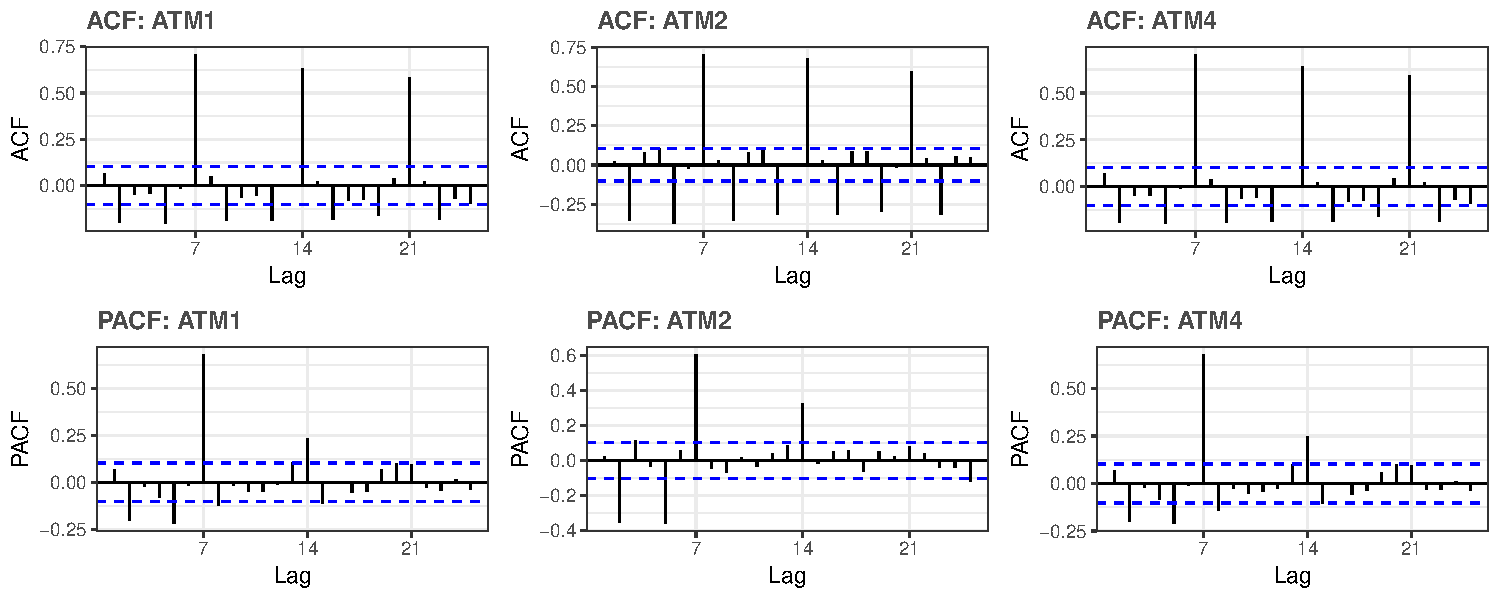
\includegraphics{Part-B-AS.final.firstparameter_files/figure-latex/unnamed-chunk-4-1.pdf}

\begin{verbatim}
FALSE 
FALSE   Ljung-Box test
FALSE 
FALSE data:  Residuals from ARIMA(3,0,2)(2,1,0)[12] with drift
FALSE Q* = 12.555, df = 16, p-value = 0.705
FALSE 
FALSE Model df: 8.   Total lags used: 24
\end{verbatim}

\subsection{Model \#2: STL (no-demped) -
MNN}\label{model-2-stl-no-demped---mnn}

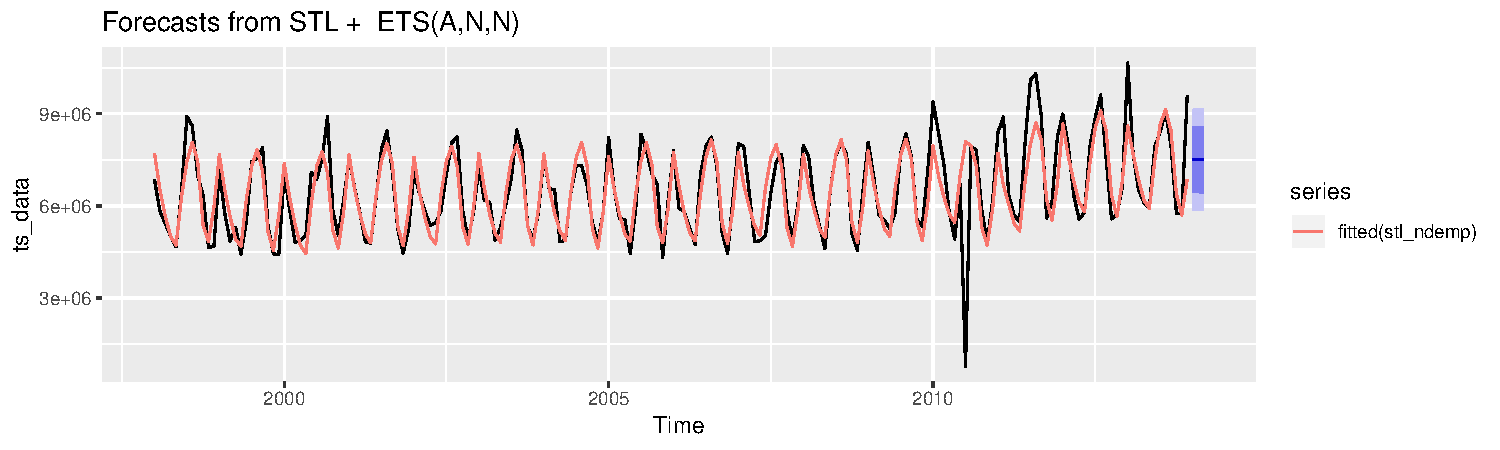
\includegraphics{Part-B-AS.final.firstparameter_files/figure-latex/unnamed-chunk-5-1.pdf}

\begin{verbatim}
FALSE 
FALSE   Ljung-Box test
FALSE 
FALSE data:  Residuals from STL +  ETS(M,N,N)
FALSE Q* = 65.934, df = 22, p-value = 2.84e-06
FALSE 
FALSE Model df: 2.   Total lags used: 24
\end{verbatim}

\subsection{Model \#2-2: STL (demped) -
MAdN}\label{model-2-2-stl-demped---madn}

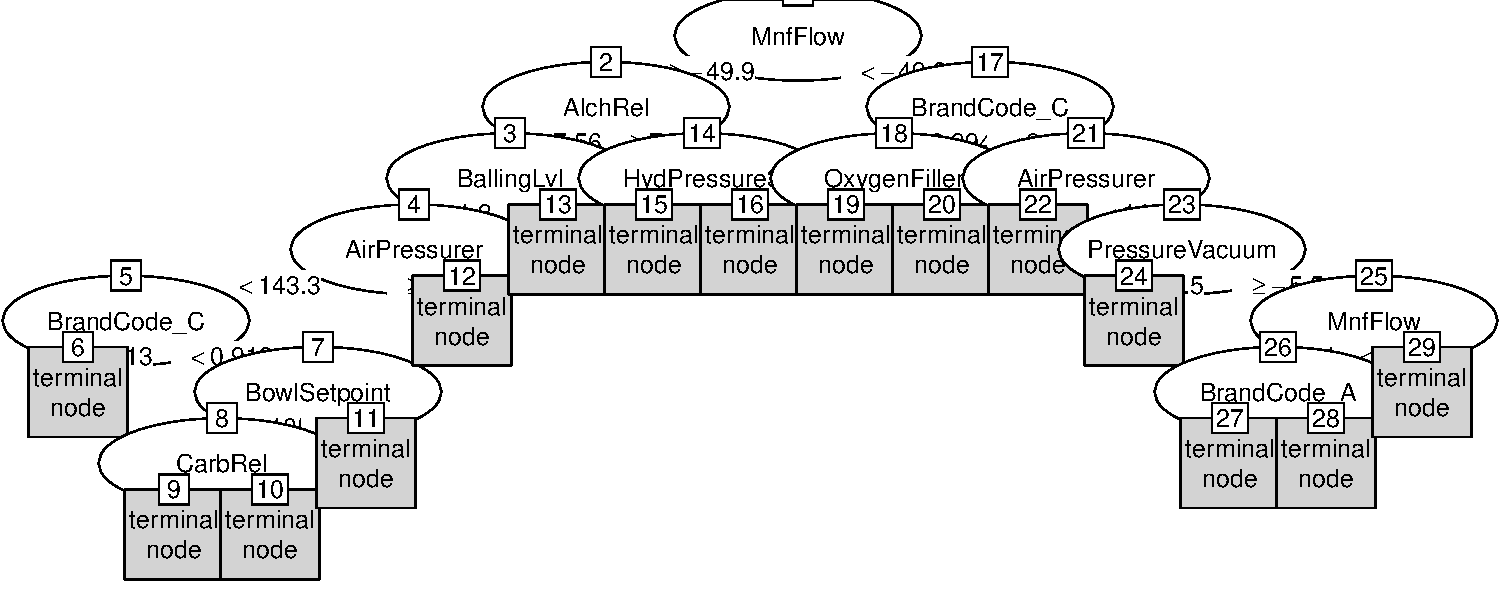
\includegraphics{Part-B-AS.final.firstparameter_files/figure-latex/unnamed-chunk-6-1.pdf}

\begin{verbatim}
FALSE 
FALSE   Ljung-Box test
FALSE 
FALSE data:  Residuals from STL +  ETS(M,Ad,N)
FALSE Q* = 63.375, df = 19, p-value = 1.119e-06
FALSE 
FALSE Model df: 5.   Total lags used: 24
\end{verbatim}

\subsection{Model \#3: ets - MNM}\label{model-3-ets---mnm}

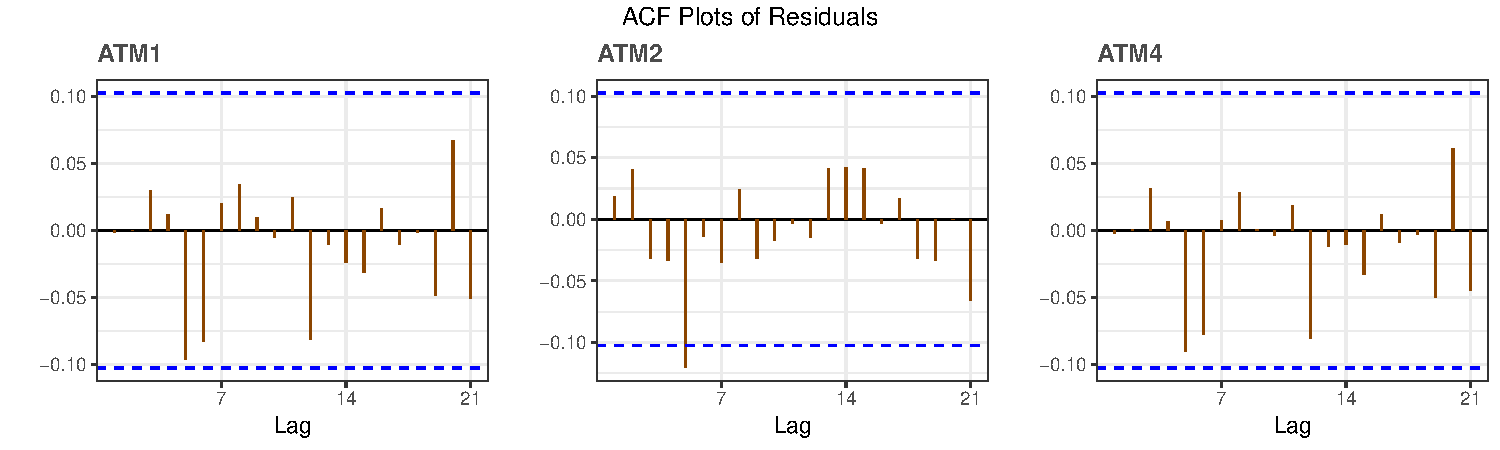
\includegraphics{Part-B-AS.final.firstparameter_files/figure-latex/unnamed-chunk-7-1.pdf}

\begin{verbatim}
FALSE 
FALSE   Ljung-Box test
FALSE 
FALSE data:  Residuals from ETS(M,N,M)
FALSE Q* = 32.042, df = 10, p-value = 0.000394
FALSE 
FALSE Model df: 14.   Total lags used: 24
\end{verbatim}

\section*{Forecast}\label{b-forecast}
\addcontentsline{toc}{section}{Forecast}

\texttt{auto.arima()} performs cross validation on hyperparameter tuning
to find the best model with parameters of \texttt{order} and
\texttt{seasonal} that minimize \texttt{AIC}. This gave us
\textbf{arima\_model}: ARIMA\((3,0,2)(2,1,0)12\) with drift resulting
\texttt{AIC} = 5332.24.

Since ARIMA is the only reliable model, as other models failed Ljung
test, we will plot forecasts of ARIMA only. The forecasted values can be
viewed in the appendix.

\subsection{Model \#1: ARIMA}\label{model-1-arima-1}

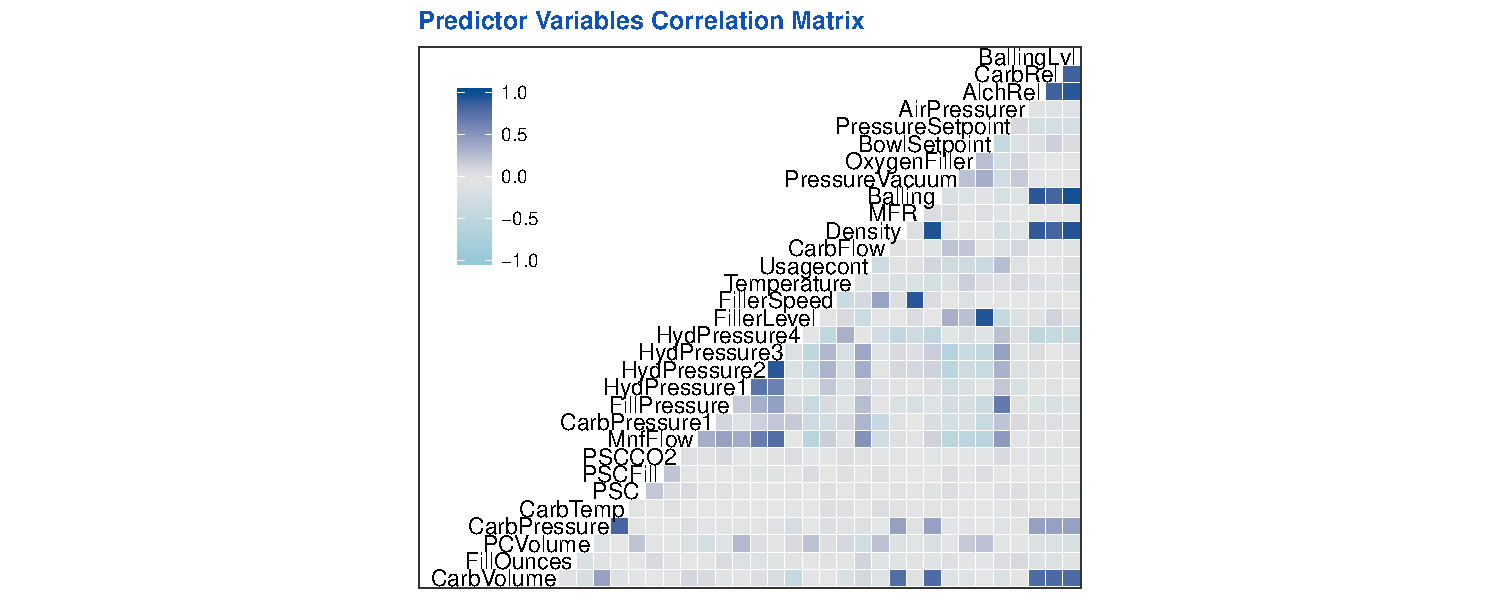
\includegraphics{Part-B-AS.final.firstparameter_files/figure-latex/unnamed-chunk-8-1.pdf}

\section*{Discussion}\label{b-discussion}
\addcontentsline{toc}{section}{Discussion}

We implemented a cross validation method of testing for h=12. The
process randomly chooses 12 points to measure and take the average of
RMSEs. By definition, a lower RMSE on test set is attributed with a
better forecast on unseen data.

Using Time series cross-validation, we compute RMSE on testset (h=12).
We would have to pick the model with the lowest RMSE on test set as our
final model if we had more than 1 model to compare. In our case, since
we only have 1 model left after Ljung test, we have no choice but to
pick seasonal ARIMA model as our final choice. Cross-validation test
shows that RMSE on test is around 720k when RMSE on training is around
589k. We can conclude the model is not necessarily overfitted. Given
that MAPE on training is less than 7, it is not a suprising result.

\begin{verbatim}
FALSE [1] "RMSE - train: 589381.7"
\end{verbatim}

\begin{verbatim}
FALSE [1] "RMSE - test: 725175"
\end{verbatim}

\chapter*{Appendix}\label{Appendix}
\addcontentsline{toc}{chapter}{Appendix}

\section*{Part B}\label{Part-B}
\addcontentsline{toc}{section}{Part B}

\subsection*{Model Summary}\label{Part-B-summary}
\addcontentsline{toc}{subsection}{Model Summary}

\textbf{\texttt{ARIMA}:}

\begin{verbatim}
FALSE 
FALSE Forecast method: ARIMA(3,0,2)(2,1,0)[12] with drift
FALSE 
FALSE Model Information:
FALSE Series: ts_data_o 
FALSE ARIMA(3,0,2)(2,1,0)[12] with drift 
FALSE 
FALSE Coefficients:
FALSE           ar1      ar2     ar3     ma1     ma2     sar1     sar2     drift
FALSE       -0.5606  -0.2216  0.3284  0.8902  0.4827  -0.7249  -0.4152  9018.405
FALSE s.e.   0.3992   0.3382  0.0960  0.4120  0.4551   0.0797   0.0841  3027.685
FALSE 
FALSE sigma^2 estimated as 3.878e+11:  log likelihood=-2657.12
FALSE AIC=5332.24   AICc=5333.3   BIC=5360.97
FALSE 
FALSE Error measures:
FALSE                     ME     RMSE      MAE        MPE     MAPE      MASE
FALSE Training set -8455.077 589381.7 427752.5 -0.7944782 6.475365 0.6904053
FALSE                      ACF1
FALSE Training set 0.0006090194
FALSE 
FALSE Forecasts:
FALSE          Point Forecast   Lo 80    Hi 80   Lo 95    Hi 95
FALSE Jan 2014       10210619 9412589 11008649 8990138 11431100
FALSE Feb 2014        8722658 7882412  9562903 7437613 10007702
FALSE Mar 2014        7137962 6295514  7980411 5849548  8426376
FALSE Apr 2014        5919874 5060514  6779234 4605596  7234152
FALSE May 2014        5946730 5087082  6806377 4632012  7261448
FALSE Jun 2014        8383812 7524148  9243475 7069070  9698553
FALSE Jul 2014        9362213 8500206 10224219 8043888 10680538
FALSE Aug 2014       10018953 9155935 10881971 8699080 11338826
FALSE Sep 2014        8547612 7684559  9410664 7227687  9867536
FALSE Oct 2014        5781906 4918467  6645344 4461391  7102421
FALSE Nov 2014        6193673 5329717  7057629 4872367  7514980
FALSE Dec 2014        8373767 7509705  9237829 7052298  9695236
\end{verbatim}

\textbf{\texttt{STL\ -\ MNN}:}

\begin{verbatim}
FALSE 
FALSE Forecast method: STL +  ETS(M,N,N)
FALSE 
FALSE Model Information:
FALSE ETS(M,N,N) 
FALSE 
FALSE Call:
FALSE  ets(y = x, model = etsmodel, allow.multiplicative.trend = allow.multiplicative.trend) 
FALSE 
FALSE   Smoothing parameters:
FALSE     alpha = 0.1159 
FALSE 
FALSE   Initial states:
FALSE     l = 6317745.8917 
FALSE 
FALSE   sigma:  0.097
FALSE 
FALSE      AIC     AICc      BIC 
FALSE 6139.631 6139.758 6149.403 
FALSE 
FALSE Error measures:
FALSE                    ME     RMSE      MAE         MPE     MAPE      MASE
FALSE Training set 56926.03 633571.7 460713.4 -0.03288687 6.945185 0.7436052
FALSE                   ACF1
FALSE Training set 0.2570241
FALSE 
FALSE Forecasts:
FALSE          Point Forecast   Lo 80    Hi 80   Lo 95    Hi 95
FALSE Jan 2014        8992609 8049591  9935628 7550387 10434831
FALSE Feb 2014        7908116 6958724  8857508 6456146  9360086
FALSE Mar 2014        7079434 6123709  8035158 5617779  8541088
FALSE Apr 2014        6435209 5473193  7397225 4963933  7906486
FALSE May 2014        6161593 5193326  7129860 4680756  7642430
FALSE Jun 2014        7728705 6754226  8703185 6238368  9219043
FALSE Jul 2014        8837980 7857327  9818633 7338201 10337759
FALSE Aug 2014        9376841 8390053 10363630 7867678 10886004
FALSE Sep 2014        8601001 7608114  9593888 7082511 10119490
FALSE Oct 2014        6670419 5671470  7669368 5142658  8198180
FALSE Nov 2014        6035845 5030870  7040821 4498868  7572822
FALSE Dec 2014        7189087 6178120  8200053 5642947  8735226
\end{verbatim}

\textbf{\texttt{STL\ -\ MAdN}:}

\begin{verbatim}
FALSE 
FALSE Forecast method: STL +  ETS(M,Ad,N)
FALSE 
FALSE Model Information:
FALSE ETS(M,Ad,N) 
FALSE 
FALSE Call:
FALSE  ets(y = x, model = etsmodel, damped = TRUE, allow.multiplicative.trend = allow.multiplicative.trend) 
FALSE 
FALSE   Smoothing parameters:
FALSE     alpha = 0.1233 
FALSE     beta  = 1e-04 
FALSE     phi   = 0.8 
FALSE 
FALSE   Initial states:
FALSE     l = 5615471.7851 
FALSE     b = 173606.4508 
FALSE 
FALSE   sigma:  0.0972
FALSE 
FALSE      AIC     AICc      BIC 
FALSE 6143.452 6143.906 6162.997 
FALSE 
FALSE Error measures:
FALSE                    ME     RMSE      MAE         MPE     MAPE      MASE
FALSE Training set 54337.68 631081.9 458777.5 -0.07364717 6.937249 0.7404807
FALSE                   ACF1
FALSE Training set 0.2528558
FALSE 
FALSE Forecasts:
FALSE          Point Forecast   Lo 80    Hi 80   Lo 95    Hi 95
FALSE Jan 2014        9007707 8060947  9954467 7559763 10455651
FALSE Feb 2014        7923348 6969325  8877372 6464295  9382401
FALSE Mar 2014        7094774 6133536  8056011 5624687  8564860
FALSE Apr 2014        6450635 5482232  7419038 4969591  7931680
FALSE May 2014        6177088 5201569  7152607 4685160  7669016
FALSE Jun 2014        7744256 6761668  8726843 6241518  9246993
FALSE Jul 2014        8853574 7863967  9843182 7340100 10367048
FALSE Aug 2014        9392471 8395890 10389052 7868332 10916609
FALSE Sep 2014        8616658 7613151  9620166 7081926 10151391
FALSE Oct 2014        6686100 5675711  7696488 5140843  8231356
FALSE Nov 2014        6051544 5034319  7068769 4495832  7607255
FALSE Dec 2014        7204799 6180782  8228817 5638700  8770899
\end{verbatim}

\textbf{\texttt{ets\ -\ MNM}:}

\begin{verbatim}
FALSE 
FALSE Forecast method: ETS(M,N,M)
FALSE 
FALSE Model Information:
FALSE ETS(M,N,M) 
FALSE 
FALSE Call:
FALSE  ets(y = ts_data_o) 
FALSE 
FALSE   Smoothing parameters:
FALSE     alpha = 0.1428 
FALSE     gamma = 0.2119 
FALSE 
FALSE   Initial states:
FALSE     l = 6189149.8743 
FALSE     s = 0.8984 0.7596 0.938 1.2229 1.2597 1.2396
FALSE            1.0059 0.7638 0.8078 0.8864 1.0269 1.191
FALSE 
FALSE   sigma:  0.0967
FALSE 
FALSE      AIC     AICc      BIC 
FALSE 6144.033 6146.760 6192.895 
FALSE 
FALSE Error measures:
FALSE                    ME     RMSE      MAE         MPE     MAPE      MASE
FALSE Training set 45241.77 628252.5 481520.9 -0.04000239 7.277118 0.7771892
FALSE                   ACF1
FALSE Training set 0.1927438
FALSE 
FALSE Forecasts:
FALSE          Point Forecast   Lo 80    Hi 80   Lo 95    Hi 95
FALSE Jan 2014        9917654 8689211 11146096 8038913 11796394
FALSE Feb 2014        8522973 7456477  9589469 6891908 10154038
FALSE Mar 2014        7012478 6126191  7898765 5657019  8367937
FALSE Apr 2014        6208601 5416196  7001006 4996722  7420480
FALSE May 2014        5928833 5164834  6692832 4760398  7097269
FALSE Jun 2014        7840532 6820624  8860440 6280717  9400347
FALSE Jul 2014        9115823 7919004 10312642 7285446 10946200
FALSE Aug 2014        9648549 8370229 10926869 7693527 11603571
FALSE Sep 2014        8553364 7409986  9696742 6804718 10302010
FALSE Oct 2014        6266745 5421655  7111835 4974291  7559199
FALSE Nov 2014        5938289 5130560  6746017 4702975  7173603
FALSE Dec 2014        8020901 6920610  9121192 6338151  9703651
\end{verbatim}

\newpage

\subsection*{R Script}\label{Part-B-RScript}
\addcontentsline{toc}{subsection}{R Script}

\begin{Shaded}
\begin{Highlighting}[]
\CommentTok{# Dependencies}
\NormalTok{## processing}
\KeywordTok{library}\NormalTok{(readxl)}
\KeywordTok{library}\NormalTok{(tinytex)}
\KeywordTok{library}\NormalTok{(readr)}

\NormalTok{## graphs}
\KeywordTok{library}\NormalTok{(ggplot2)}
\KeywordTok{library}\NormalTok{(janitor)}
\KeywordTok{library}\NormalTok{(gridExtra)}
\KeywordTok{library}\NormalTok{(grid)}

\NormalTok{## formatting}
\KeywordTok{library}\NormalTok{(default)}
\KeywordTok{library}\NormalTok{(knitr)}
\KeywordTok{library}\NormalTok{(kableExtra)}
\KeywordTok{library}\NormalTok{(tidyverse)}
\KeywordTok{library}\NormalTok{(scales)}
\KeywordTok{library}\NormalTok{(readxl)}
\KeywordTok{library}\NormalTok{(lubridate)}

\NormalTok{## forecasting packages}
\KeywordTok{library}\NormalTok{(fpp2)}
\KeywordTok{library}\NormalTok{(forecast)}

\NormalTok{## outlier & imputation}
\KeywordTok{library}\NormalTok{(imputeTS)}
\KeywordTok{library}\NormalTok{(tsoutliers)}

\CommentTok{# load data}
\NormalTok{power_data <-}\StringTok{ }\KeywordTok{read_csv}\NormalTok{(}\StringTok{"https://raw.githubusercontent.com/vindication09/DATA-624/master/ResidentialCustomerForecastLoad-624.csv"}\NormalTok{)}

\CommentTok{# Time Series}
\NormalTok{ts_data <-}\StringTok{ }\KeywordTok{ts}\NormalTok{(power_data}\OperatorTok{$}\NormalTok{KWH, }\DataTypeTok{frequency =} \DecValTok{12}\NormalTok{, }\DataTypeTok{start =} \KeywordTok{c}\NormalTok{(}\DecValTok{1998}\NormalTok{,}\DecValTok{1}\NormalTok{))}

\CommentTok{# Missing value imputation}
\NormalTok{ts_data <-}\StringTok{ }\KeywordTok{na_interpolation}\NormalTok{(ts_data)}

\CommentTok{# STL decomposition}
\NormalTok{stl1 <-}\StringTok{ }\KeywordTok{stl}\NormalTok{(ts_data, }\DataTypeTok{s.window =} \StringTok{'periodic'}\NormalTok{)}

\CommentTok{# Handling outlier}
\NormalTok{outlier_func <-}\StringTok{ }\KeywordTok{tsoutliers}\NormalTok{(ts_data, }\DataTypeTok{iterate =} \DecValTok{2}\NormalTok{, }\DataTypeTok{lambda =} \StringTok{"auto"}\NormalTok{)}

\CommentTok{# Time Series - After outlier and imputation handeled}
\NormalTok{ts_data_o <-}\StringTok{ }\NormalTok{ts_data  }\CommentTok{# Let's treate outlier handled data seperatly for Modelling part.}
\NormalTok{ts_data_o[outlier_func}\OperatorTok{$}\NormalTok{index] <-}\StringTok{ }\NormalTok{outlier_func}\OperatorTok{$}\NormalTok{replacements}

\CommentTok{# Model#1: ARIMA}
\NormalTok{arima_auto <-}\StringTok{ }\KeywordTok{auto.arima}\NormalTok{(ts_data_o)}
\NormalTok{arima_model <-}\StringTok{ }\KeywordTok{forecast}\NormalTok{(arima_auto, }\DataTypeTok{h=}\DecValTok{12}\NormalTok{)}

\CommentTok{# Model #2: STL (no-demped) - MNN}
\NormalTok{stl_ndemp <-}\StringTok{ }\KeywordTok{stlf}\NormalTok{(ts_data_o, }\DataTypeTok{s.window =} \StringTok{"periodic"}\NormalTok{, }\DataTypeTok{robust=}\OtherTok{TRUE}\NormalTok{, }\DataTypeTok{h =} \DecValTok{12}\NormalTok{)}

\CommentTok{# Model #2-2: STL (demped) - MAdN}
\NormalTok{stl_demp <-}\StringTok{ }\KeywordTok{stlf}\NormalTok{(ts_data_o, }\DataTypeTok{damped=}\OtherTok{TRUE}\NormalTok{, }\DataTypeTok{s.window =} \StringTok{"periodic"}\NormalTok{, }\DataTypeTok{robust=}\OtherTok{TRUE}\NormalTok{, }\DataTypeTok{h =} \DecValTok{12}\NormalTok{)}

\CommentTok{# Model #3: ets - MNM}
\NormalTok{ets_auto <-}\StringTok{ }\KeywordTok{ets}\NormalTok{(ts_data_o)}
\NormalTok{ets_model <-}\StringTok{ }\KeywordTok{forecast}\NormalTok{(ets_auto, }\DataTypeTok{h=}\DecValTok{12}\NormalTok{)}

\CommentTok{# tsCv - ARIMA -> it takes so much time. I got the results and saved them}
\NormalTok{##arima_cv <- function(x, h)\{forecast(Arima(x, order = c(3, 0, 2), seasonal = c(2, 1, 0), include.drift = TRUE), h=h)\}}
\NormalTok{##e <- tsCV(ts_data_o, arima_cv, h=12)}

\CommentTok{# RMSEs -> tsCV takes lot of time to process so just saved the output}
\CommentTok{#rmse_train_arima <- arima_auto[2]}
\CommentTok{#rmse_test_arima <- sqrt(mean(e^2, na.rm=TRUE))}

\NormalTok{rmse_train_arima <-}\StringTok{ }\FloatTok{589381.7}
\NormalTok{rmse_test_arima <-}\StringTok{ }\DecValTok{725175}

\CommentTok{# Save output}
\KeywordTok{write.csv}\NormalTok{(arima_model, }\DataTypeTok{file=}\StringTok{"forecasts/POWER_ARIMA_FC.csv"}\NormalTok{)}
\end{Highlighting}
\end{Shaded}


\end{document}
